\begin{figure}
\centering

\begin{tikzpicture}

% ═══════════════════════════════════════════════════════════════════════════
%  ROW 0 – column headers
% ═══════════════════════════════════════════════════════════════════════════
\node[colhead=popclr, yshift=0.2cm]  (h1) at (\colA, \rowHead)
  {Population-level~$(\hyperparams)$};
\node[colhead=hidclr, yshift=0.2cm]  (h2) at (\colB, \rowHead)
  {Hidden parameters~$(\hiddenparams)$};
\node[colhead=dataclr, yshift=0.5cm] (h3) at (\colC, \rowHead)
  {Data~$(\datanoisy)$};

% ═════════════════════════════════════════════════════════════════════════
%  ROW 1 – generative direction
% ══════════════════════════════════════════════════════════════════════════════════════
\node[plotbox=popclr]  (p1) at (\colA, \rowOne)
  {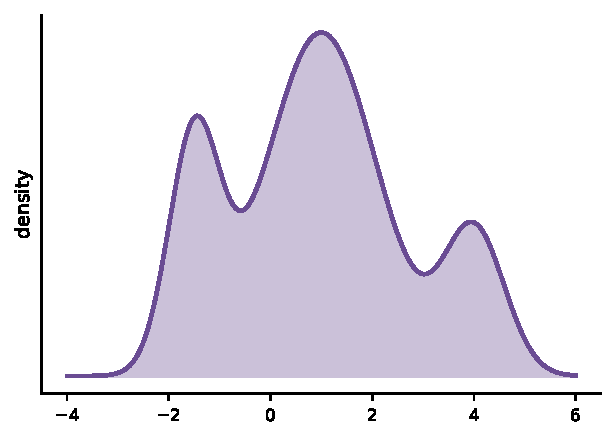
\includegraphics[width=3.0cm]{../notebooks/plots/pop_distribution.pdf}};
\node[sublabel=popclr, below=0.12cm of p1] (l1)
  {$p(\hiddenparams\mid\hyperparams)$};

\node[plotbox=hidclr]  (p2) at (\colB, \rowOne)
  {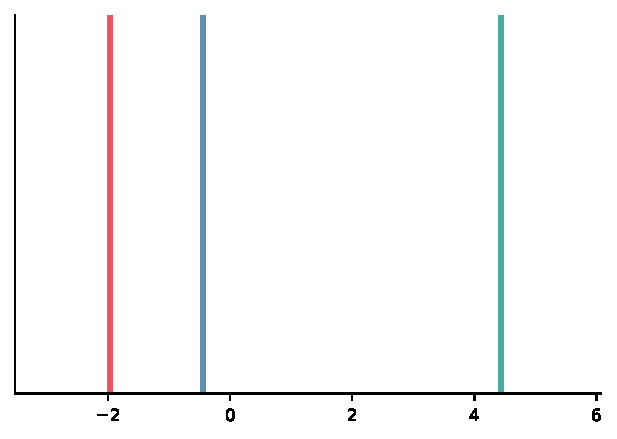
\includegraphics[width=3.0cm]{../notebooks/plots/hidden_params.pdf}};
\node[sublabel=hidclr, below=0.12cm of p2] (l2)
  {$\hiddenparam{i}\sim\prior(\cdot\mid\hyperparams)$};

\node[plotbox=dataclr] (p3) at (\colC, \rowOne)
  {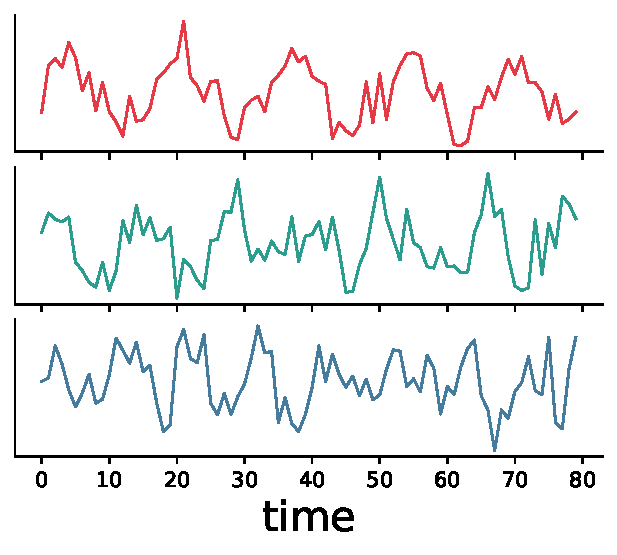
\includegraphics[width=3.0cm]{../notebooks/plots/time_series.pdf}};
\node[sublabel=dataclr, below=0.12cm of p3] (l3)
  {$\datanoisyi\!\sim\!\Lik(\cdot\mid\hiddenparam{i})$};

% ── Row-1 arrows: routed ABOVE the boxes via a lifted waypoint ───────────
\draw[arr]
  (p1.east) -- (p2.west)
  node[midway, above=4pt, font=\scriptsize, text=arrowclr] {};
    % {$\hiddenparam{i}\!\sim\!\prior(\cdot\mid\hyperparams)$};

\draw[arr]
  (p2.east) -- (p3.west)
  node[midway, above=4pt, font=\scriptsize, text=arrowclr]
    {};

% ═══════════════════════════════════════════════════════════════════════════
%  ROW 2 – inference direction
% ═══════════════════════════════════════════════════════════════════════════
\node[plotbox=hidclr]  (post) at (\colB, \rowTwo)
  {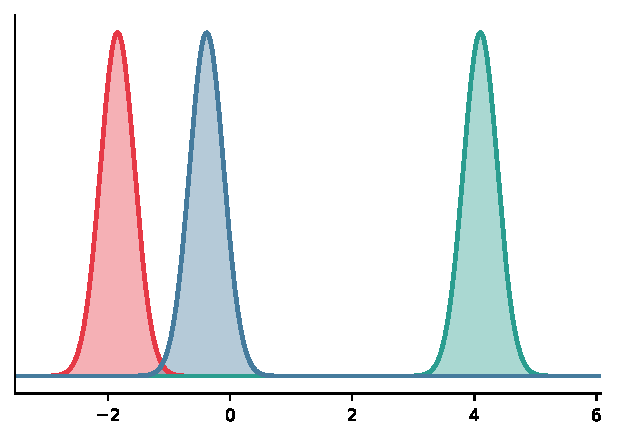
\includegraphics[width=3.0cm]{../notebooks/plots/posteriors.pdf}};
\node[sublabel=hidclr, below=0.12cm of post] (lpost)
{\shortstack{Single-event posteriors \\ $\prior(\hiddenparam{i}\mid\datanoisyi)$}};

\node[plotbox=ppclr]   (pp)   at (\colA, \rowTwo)
  {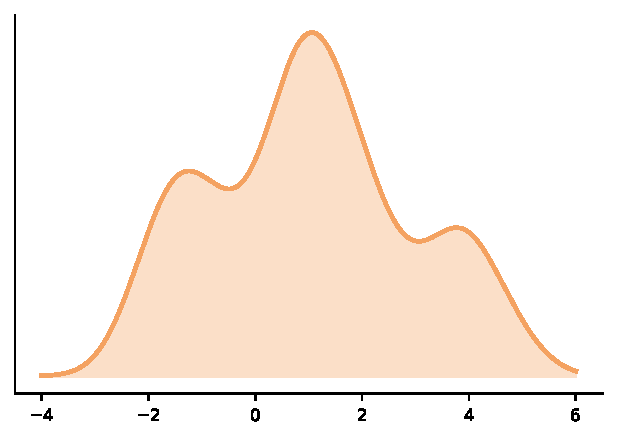
\includegraphics[width=3.0cm]{../notebooks/plots/posterior_predictive.pdf}};
\node[sublabel=ppclr, below=0.12cm of pp] (lpp)
  {\shortstack{Posterior predictive \\ $p(Y \mid \mathbf{Z})$}};

% ── Diagonal arrow: data → posteriors
%    Route: go south from p3, then west-and-south via two waypoints,
%    arriving from the right of (post) — never crossing any box interior.
\coordinate (wp1) at ($(p3.south) + (0, -1.0cm)$);   % below data box
\coordinate (wp2) at ($(post.east) + (1.8cm, 0)$);    % right of posterior box

\draw[arr, color=hidclr!70!black]
    (wp1)
    -- (wp2)
    -- (post.east)
  node[pos=0.55, right=50pt, font=\scriptsize,
       text=hidclr!70!black, align=left]
    {};

% ── Arrow: posteriors → posterior predictive (horizontal, below row labels)
\draw[arr, color=ppclr!80!black]
  (post.west) -- (pp.east)
  node[midway, above=4pt, font=\scriptsize, text=ppclr!80!black]
    {};

% ── Dashed feedback: posteriors → population prior
%    Route west then north, arriving at bottom of p1, staying left of all boxes
\coordinate (fb1) at ($(post.south) + (0, -0.8cm)$);          % below post
\coordinate (fb2) at ($(pp.south)   + (0, -0.8cm)$);          % below pp
\coordinate (fb3) at ($(p1.south)   + (0, -0.8cm)$);          % below p1

% ═══════════════════════════════════════════════════════════════════════════
%  Background column shading
% ═══════════════════════════════════════════════════════════════════════════
\begin{scope}[on background layer]
  \node[fit=(h1)(p1)(l1)(pp)(lpp),
        fill=popclr!5, rounded corners=6pt, inner sep=10pt] {};
  \node[fit=(h2)(p2)(l2)(post)(lpost),
        fill=hidclr!5, rounded corners=6pt, inner sep=10pt] {};
  \node[fit=(h3)(p3)(l3),
        fill=dataclr!5, rounded corners=6pt, inner sep=10pt] {};
\end{scope}

\end{tikzpicture}
\caption{Schematic of the generative model (top row) and inference process (bottom row).}
\end{figure}
